\chapter{Redis}

Redis is an open-source in-memory data structure store implementing a key-value
database. Redis keeps the data directly in the system memory providing fast
access times. Although data in memory is volatile, Redis provides capabilities
to persist data. Redis supports multiple data structures. Redis is implemented
in the programming language C \cite{introredis}.

Furthermore there are clients for a variety of programming languages such as C,
C\#, C++, Java, Javascript, Python, PHP, Go, Swift etc \cite{clientredis}.

\section{History}
``Redis'' stands for ``Remote Dictionary Service''. In 2009 Salvatore Sanfilippo
started the development of Redis. His goal was to improve the performance and
scalability of a self-developed application. Redis itself began to grow rapidly
in popularity the next months and Sanfilippo decided to make the project
open-source. Since March 2010 Sanfilippo is working full-time on Redis at VMWare
with Redis still being open-source \cite{russoredis,wikiredis}.

\section{Data structures}
\subsection{Strings}
The most basic type in Redis is a string. Even numbers, binary data, and images
are saved as a string with a maximum length of 512 Megabytes.

\subsection{Lists}
Lists are essentially collections of string elements that are sorted based on
the insertion order. Redis lists are implemented as linked lists. Thereby adding
an element to the head or tail of the list is always performed in constant time
regardless of the length of the list. On the other hand accessing elements in
linked lists is slower because index access - as opposed to arrays - is not
possible.

\subsection{Sets}
Redis sets represent collections of unique and unsorted string elements. Adding,
removing and existence tests of members are possible in constant time.
Furthermore there are server side commands for intersections, union or
differences of sets to create new sets in short time. 

\subsection{Sorted sets}
Sorted Sets are basically sets but every element in a sorted set is associated
with a user-defined floating point value, called the score. When querying Sorted
Sets, the elements are always returned ordered by their score. This data
structure is ideal for range queries, resolving the range query limitation.

\subsection{Hashes}
Hashes are maps of fields associated to values. Hashes are ideal to represent
objects \cite{datatypesredis}.

\section{Interesting features}
\subsection{Replication}
Redis has powerful master-slave replication capabilities. Master and slave
instances can be defined. Each master can have any number of slaves which are
exact copies of the linked master. Slaves can also be linked to slaves in a
cascading-like structure. The replication works asynchronously \cite{replicaredis}.

\subsection{Partitioning}
Partitioning allows to split the data into multiple Redis instances. This is
useful for larger databases and for scaling using the memory and computational
power of several machines. Data is partitioned as subsets of the full dataset.
Every Redis instance is independent of the others. An additional software is
necessary to handle the partitioning \cite{partitionredis}.

\subsection{Persistence}
To provide persistence Redis saves data from memory to disk. Redis supports
several persistence options \cite{persistenceredis}:
\begin{itemize}
    \item Point-in-time snapshots of the dataset in specified interval.
    \item Logging each command to a file. In case of a crash the file is
    replayed.
    \item Both methods can be combined.
    \item Persistence can be deactivated if necessary.
\end{itemize}

\subsection{Expiring keys}
Redis keys can be defined with a time to live by setting a timeout on the key.
After the timer is expired the key gets automatically deleted.

\section{Redis compared to SQL databases}
Relational database systems are very strong with set operations like
intersection, union and difference. Redis was not designed for relations and set
operations in the first place, but still offers those popular SQL operations.
The Redis commands are: SINTER, SDIFF, SNUNION.

Redis provides transaction functionality like SQL. This is very useful to define
several commands as one atomic operation. In a transaction either all commands
are executed or none.

\section{Advantages}
\subsection{Performance}
Redis is really fast, because all the data resides in the memory and data is
stored in a way which is suitable for fast retrieval.

\subsection{Atomicity}
All Redis methods to manipulate the data are atomic.

\subsection{Well known data structures}
Redis supports foundational data structures which are commonly known to computer
scientists. All Redis commands are measured in big O notation. Thereby it’s easy
to understand query performance.

\section{Disadvantages}
\subsection{Memory consumption}
Redis holds all the data in memory. Therefore it uses an amount of memory which
is equivalent to the size of the data. Most cloud services are charged by memory
usage increasing cost in comparison with disk storage based databases.

\subsection{Persistence}
To be persistent Redis writes data from memory to disk and makes heavy use of
I/O operations.

\section{Fields of application}
Redis can be a good solution in a variety of application fields.

For instance, Redis can be usedpersistenceredis
\begin{itemize}
    \item for caching in high performance web applications.
    \item for supplying transient or precalculated data.
    \item for counting with the INCR method.
    \item as session store.
    \item for queueing because of its push and pop functionalities.
    \item as message broker with its built in publish and subscribe
    functionalities.
\end{itemize}
A list of popular sites using Redis can be found on techstacks.io.

\section{CAP}
\begin{figure}[h]
    \centering
    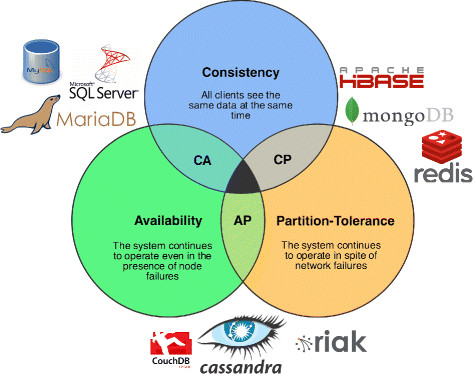
\includegraphics[width=.6\textwidth]{images/cap.png}
    \caption{Redis position in CAP}
\end{figure}
By default Redis runs as a single-server instance. It is possible to partition
Redis for example by using Redis Cluster. Only in this case the CAP-Theorem can
be applied. The full dataset then is split over all nodes. A data subset is
stored entirely onto one instance and won’t be split further by Redis. In case
of a node failure, the cluster itself remains working with the available data
still being consistent. But those subsets of data on the non-responding node are
unavailable.

Redis thus fulfills the ``CP'' of the CAP-Theorem only when running on multiple
nodes in partition mode.

\section{Conclusion}
Redis is open-source and still developed actively. It offers a well documented
API and due to its popularity there is a huge community. Redis has proven itself
and is used by a lot of major companies. Redis is offering great performance and
fast access for real-time application that don’t require complex data
operations. The desired field of application has to be well-considered whether
it is possible to trade-off functionality with performance.
